В соревнованиях по информационной безопасности задача команд найти уязвимость и эксплуатировать её, добывая секретную информацию, в нашем случае флаги. Целью модуля является прием и проверка на валидность флагов.

\subsubsection{Принцип работы}

Программа реализована с использованием вебсокетов. На порту, полученном с API, программа сравнивает IP адрес клиента с данными о IP адресах клиента или его подсети в базе данных и при нахождении его, клиент определяется как одна из команд и может отправить серверу строку. Строка проверяется на длину символов. Так же флаг проверяется на наличие в базе данных, времени его жизни (флаги валидны определенное количество времени), принадлежность другой команде (свои флаги сдавать нельзя) и статус сервиса (аналогичный сервис сдающей команды должен быть поднят). 

Ниже представлен алгоритм и наглядная схема работы flags.py

\begin{figure}[ht!]
\center{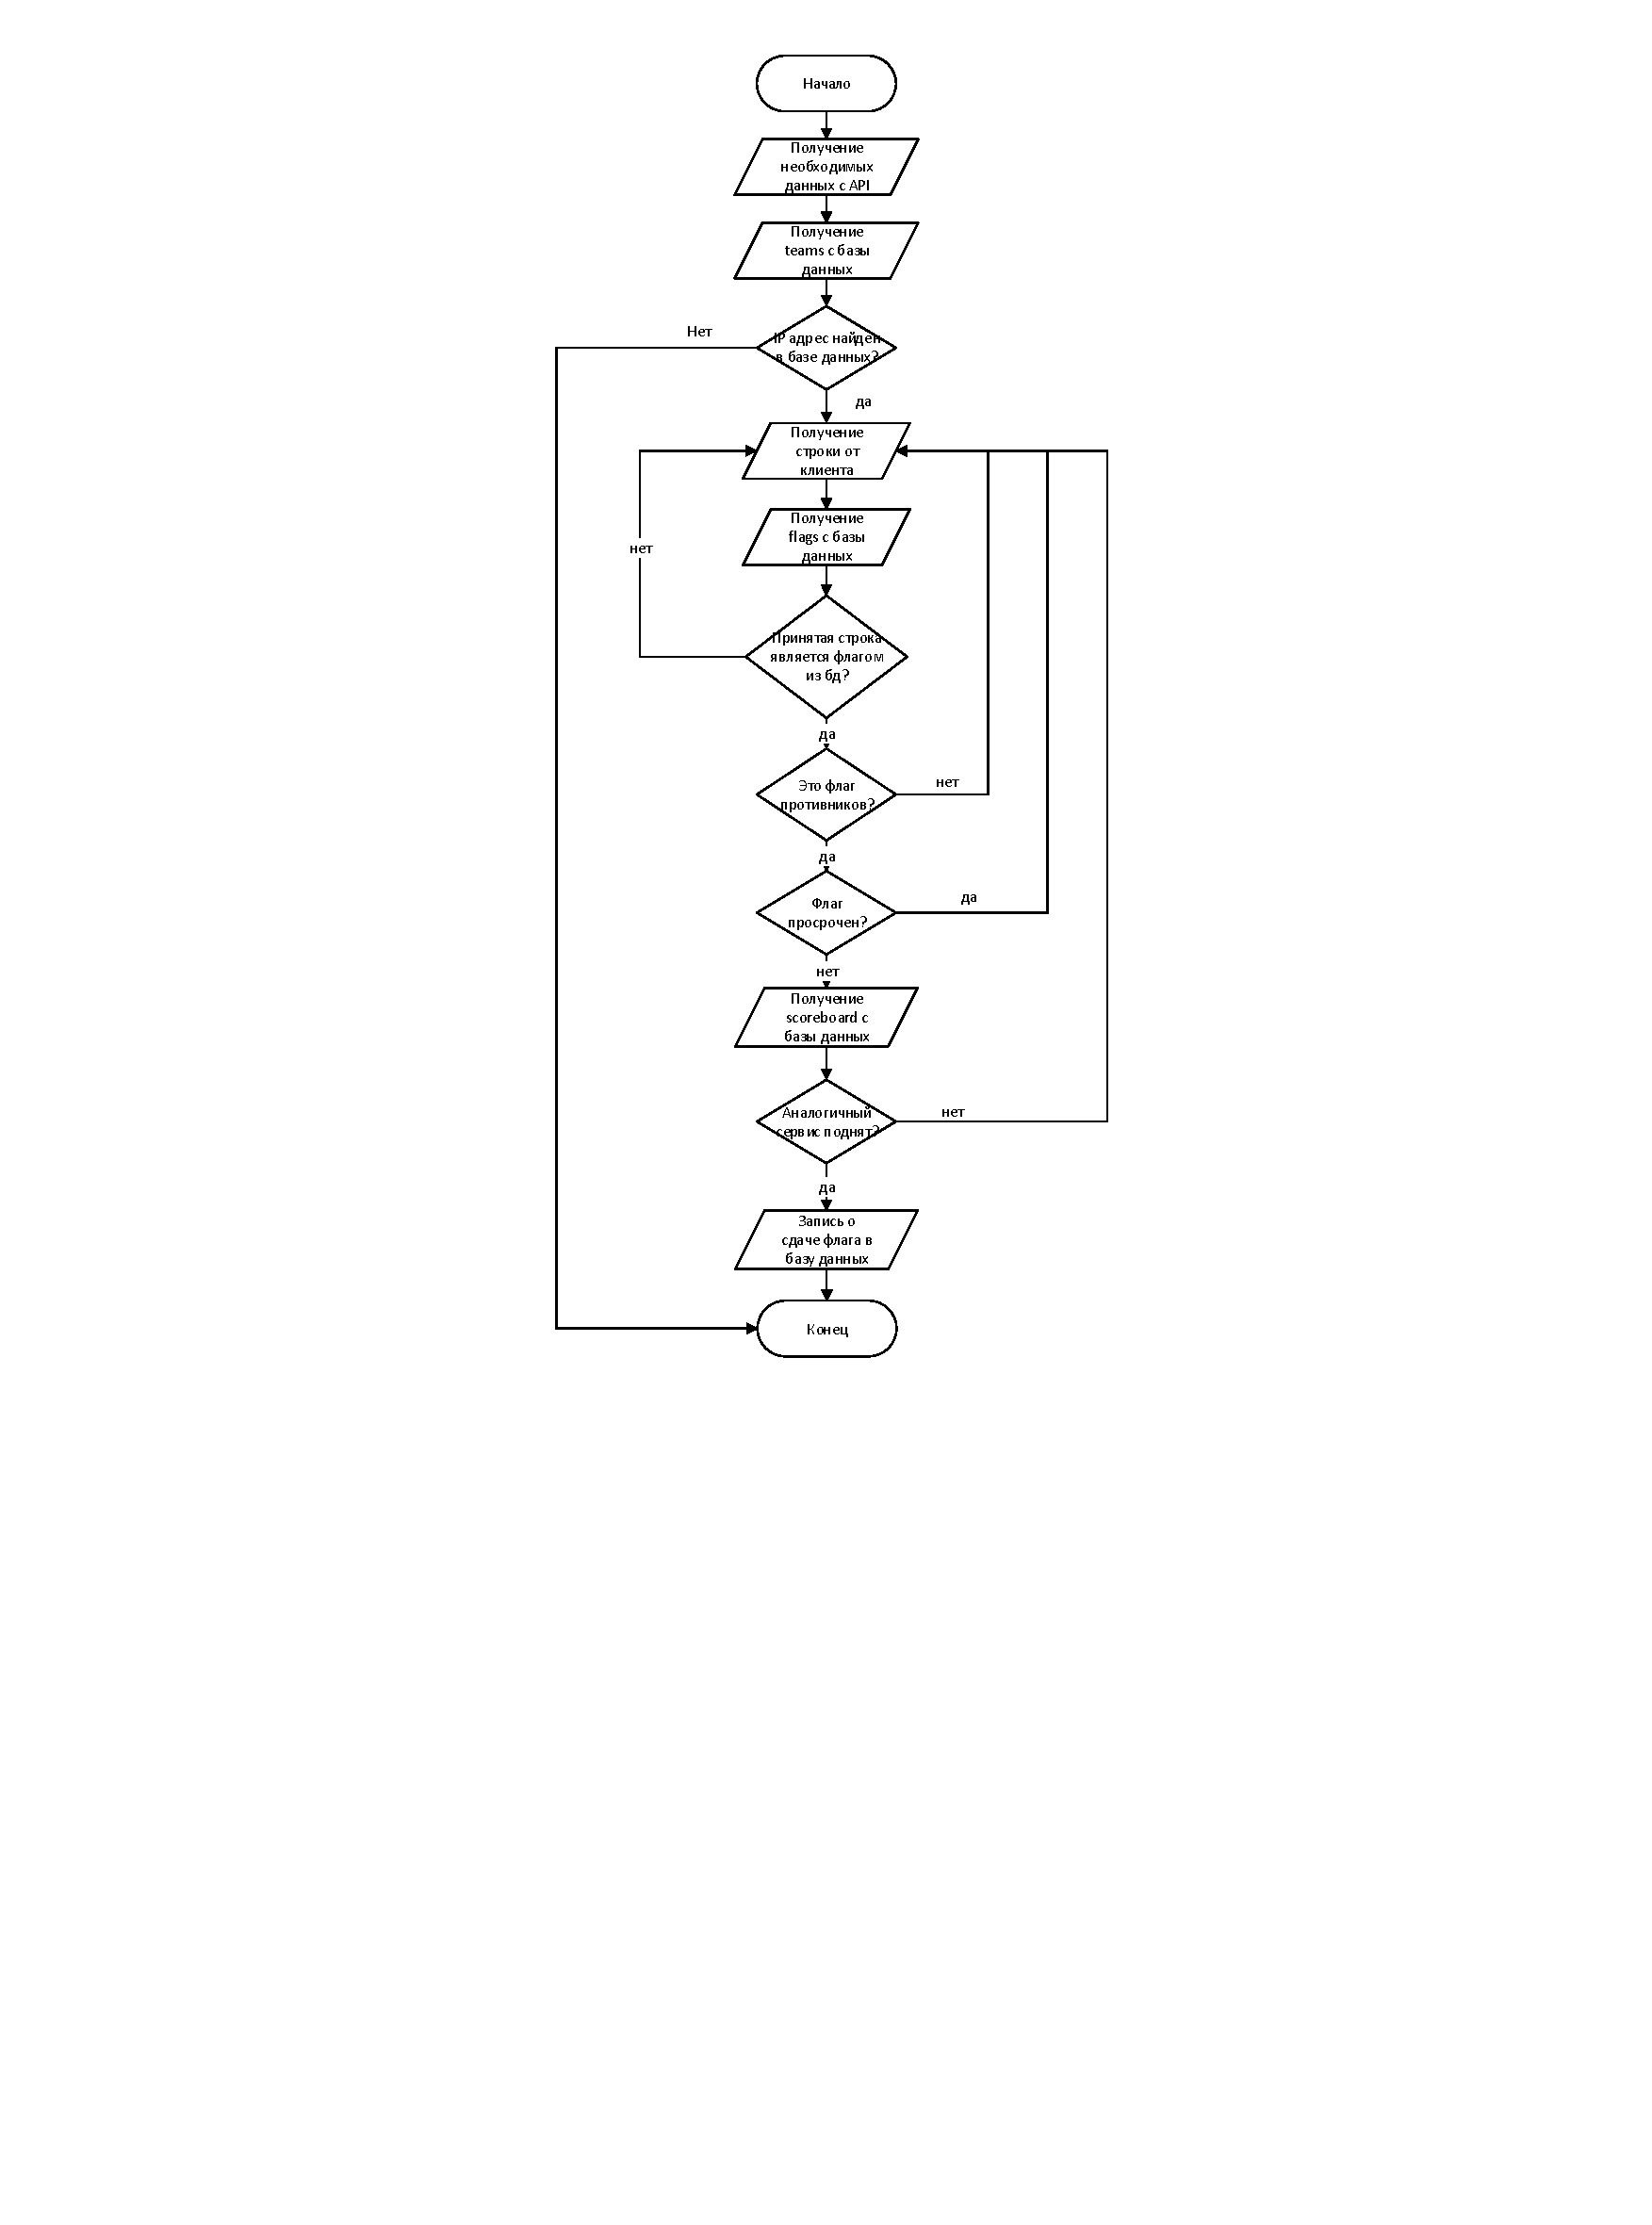
\includegraphics[trim=200 400 200 0, width=0.7\linewidth]{individual_reports/Algoritm.pdf}}
\caption{Алгоритм модуля flags.py}
\end{figure} 

\begin{figure}[ht!]
\center{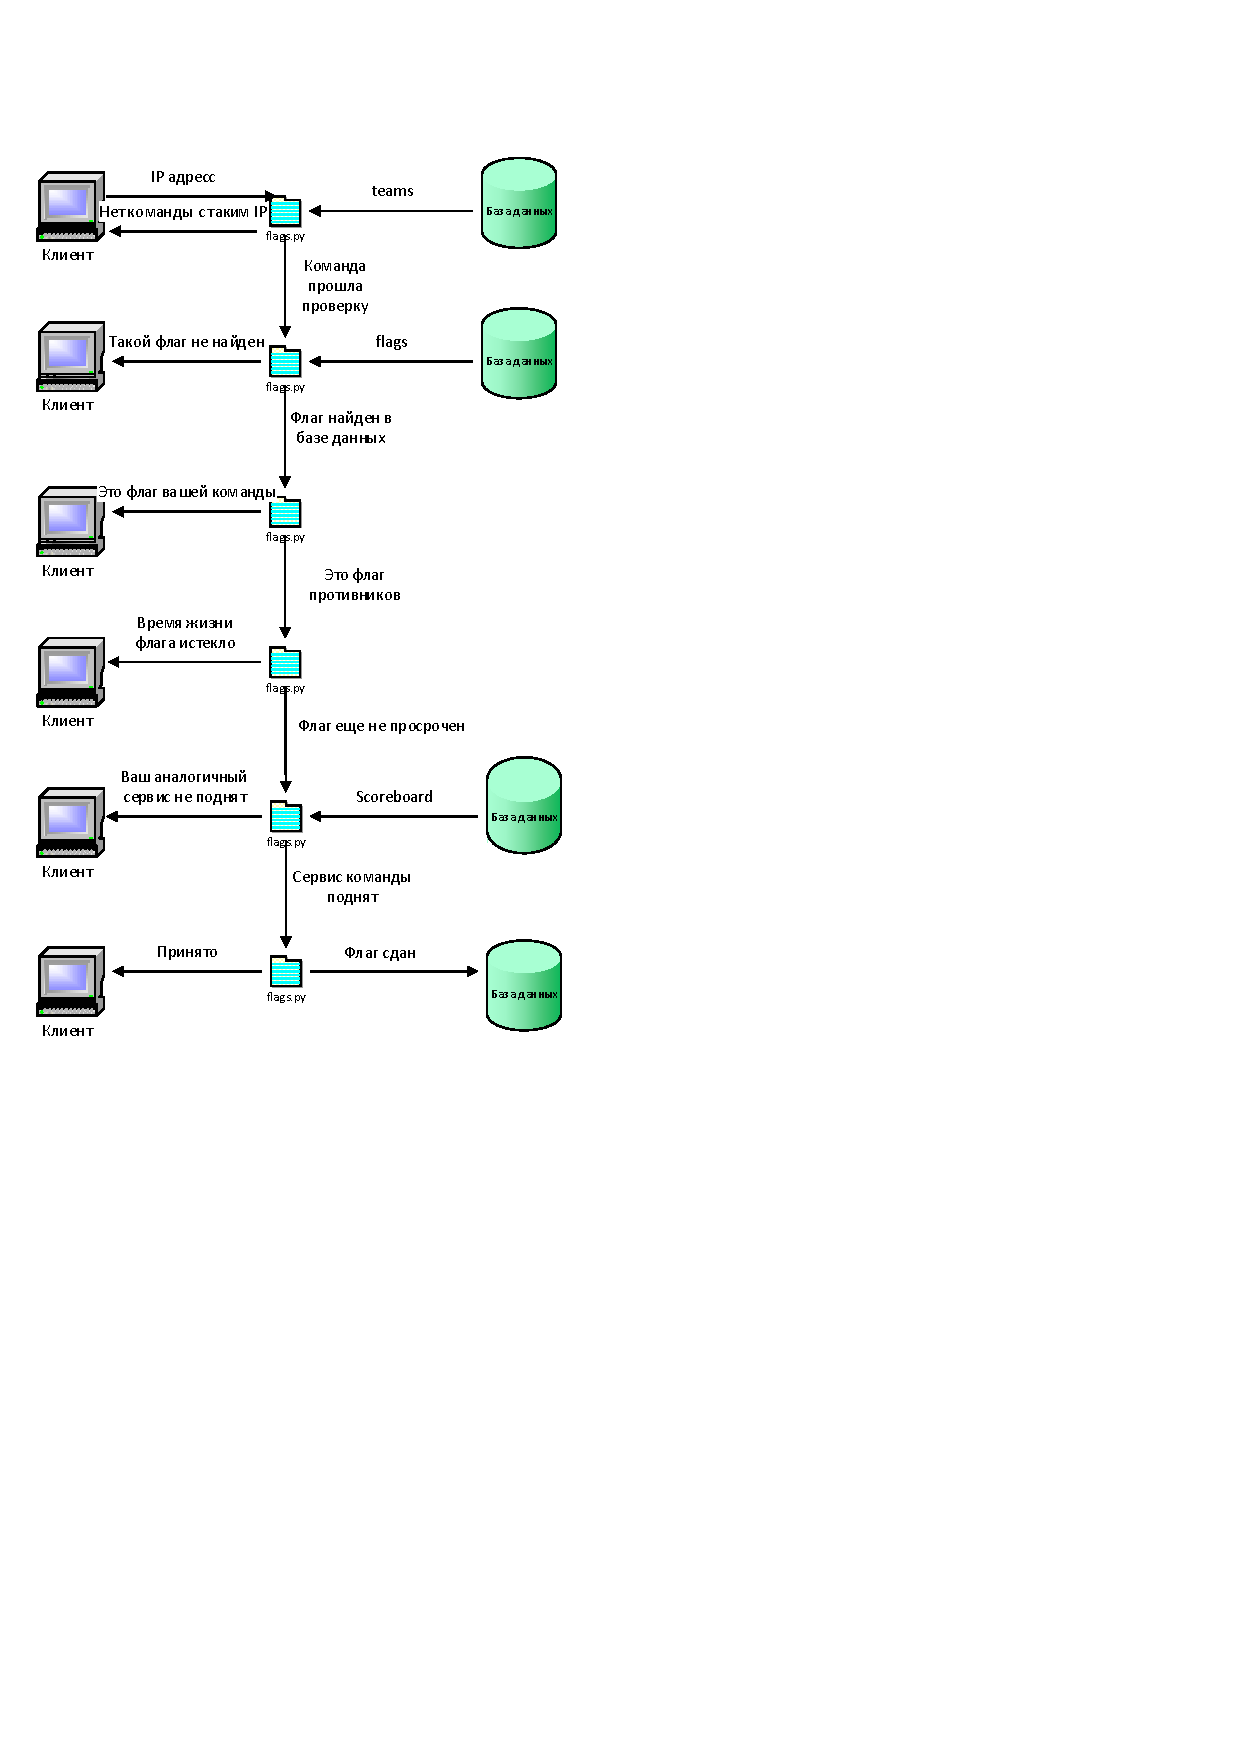
\includegraphics[trim=0 300 300 0, width=0.7\linewidth]{individual_reports/Naglyadno.pdf}}
\caption{Наглядная схема работы flags.py}
\end{figure} 

\clearpage
